%
%
%
%
%
%
%




\documentclass{beamer}
\usetheme{Copenhagen}
\usepackage[utf8]{inputenc}


%\usepackage{graphicx}
%\usepackage{subfigure}
%\usepackage{multimedia}
\usepackage{times}  % fonts are up to you
\usepackage{graphics}
\usepackage{amsmath}
\usepackage{media9}
\usepackage{hyperref}
\usepackage{psfrag}
\usepackage{pdfpages}
%\usepackage[style=authoryear]{biblatex}
%\bibliography{/Users/ali/Library/texmf/bibtex/bib/references}


\setbeamertemplate{bibliography item}[text]
%\usepackage[backend=bibtex, style=authoryear]{biblatex}
%\addbibresource{/Users/ali/Library/texmf/bibtex/bib/references.bib}
\newcommand{\customcite}[1]{\citeauthor{#1}, \citeyear{#1}}
\newcommand\smallFont{\fontsize{8}{7.2}\selectfont}   %Change font size.
\newcommand\mCite[1]{[\cite{#1}, \citetitle{#1}]}  %Prints name and title
\newcommand\FrameText[1]{
\begin{textblock*}{\paperwidth}(0pt,\textheight)
	\vspace{1.0cm}
    \raggedleft \smallFont #1
\end{textblock*}}

%Get rid of ugly copenhagen default symbol for enumerate
\setbeamertemplate{enumerate items}[default]   


% Create code text
% https://tex.stackexchange.com/questions/65291/code-snippet-in-text
\definecolor{codegray}{gray}{0.9}
\newcommand{\code}[1]{\colorbox{codegray}{\texttt{#1}}}




%Information to be included in the title page:
\title{Introduction to Slurm}
\author{Ali Snedden}
\institute{Nationwide Children's Hospital}
\date{April 19, 2019}
 
 
 
\begin{document}
 
\frame{\titlepage}




\begin{frame}
\frametitle{How to Connect}
Windows:
\begin{itemize}
    \item Open PuTTY
    \item Window Session $\Rightarrow$ Host Name field : username@10.70.250.101
    \item Click ``Open" to log in.
    \item Enter password
\end{itemize}

Mac:
\begin{itemize}
    \item Open Terminal (Finder $\Rightarrow$ Utilities $\Rightarrow$ Terminal)
    \item \code{ssh -X username@10.70.250.101}
\end{itemize}

\end{frame}


\begin{frame}
\frametitle{Cluster Architecture}
\begin{picture}(320,250)  %must be related to where it is centered
%\put(0, 70){\includegraphics[height=2.5in]{images/GPFS_File.eps}}
%\setbeamercolor{background canvas}{bg=}
%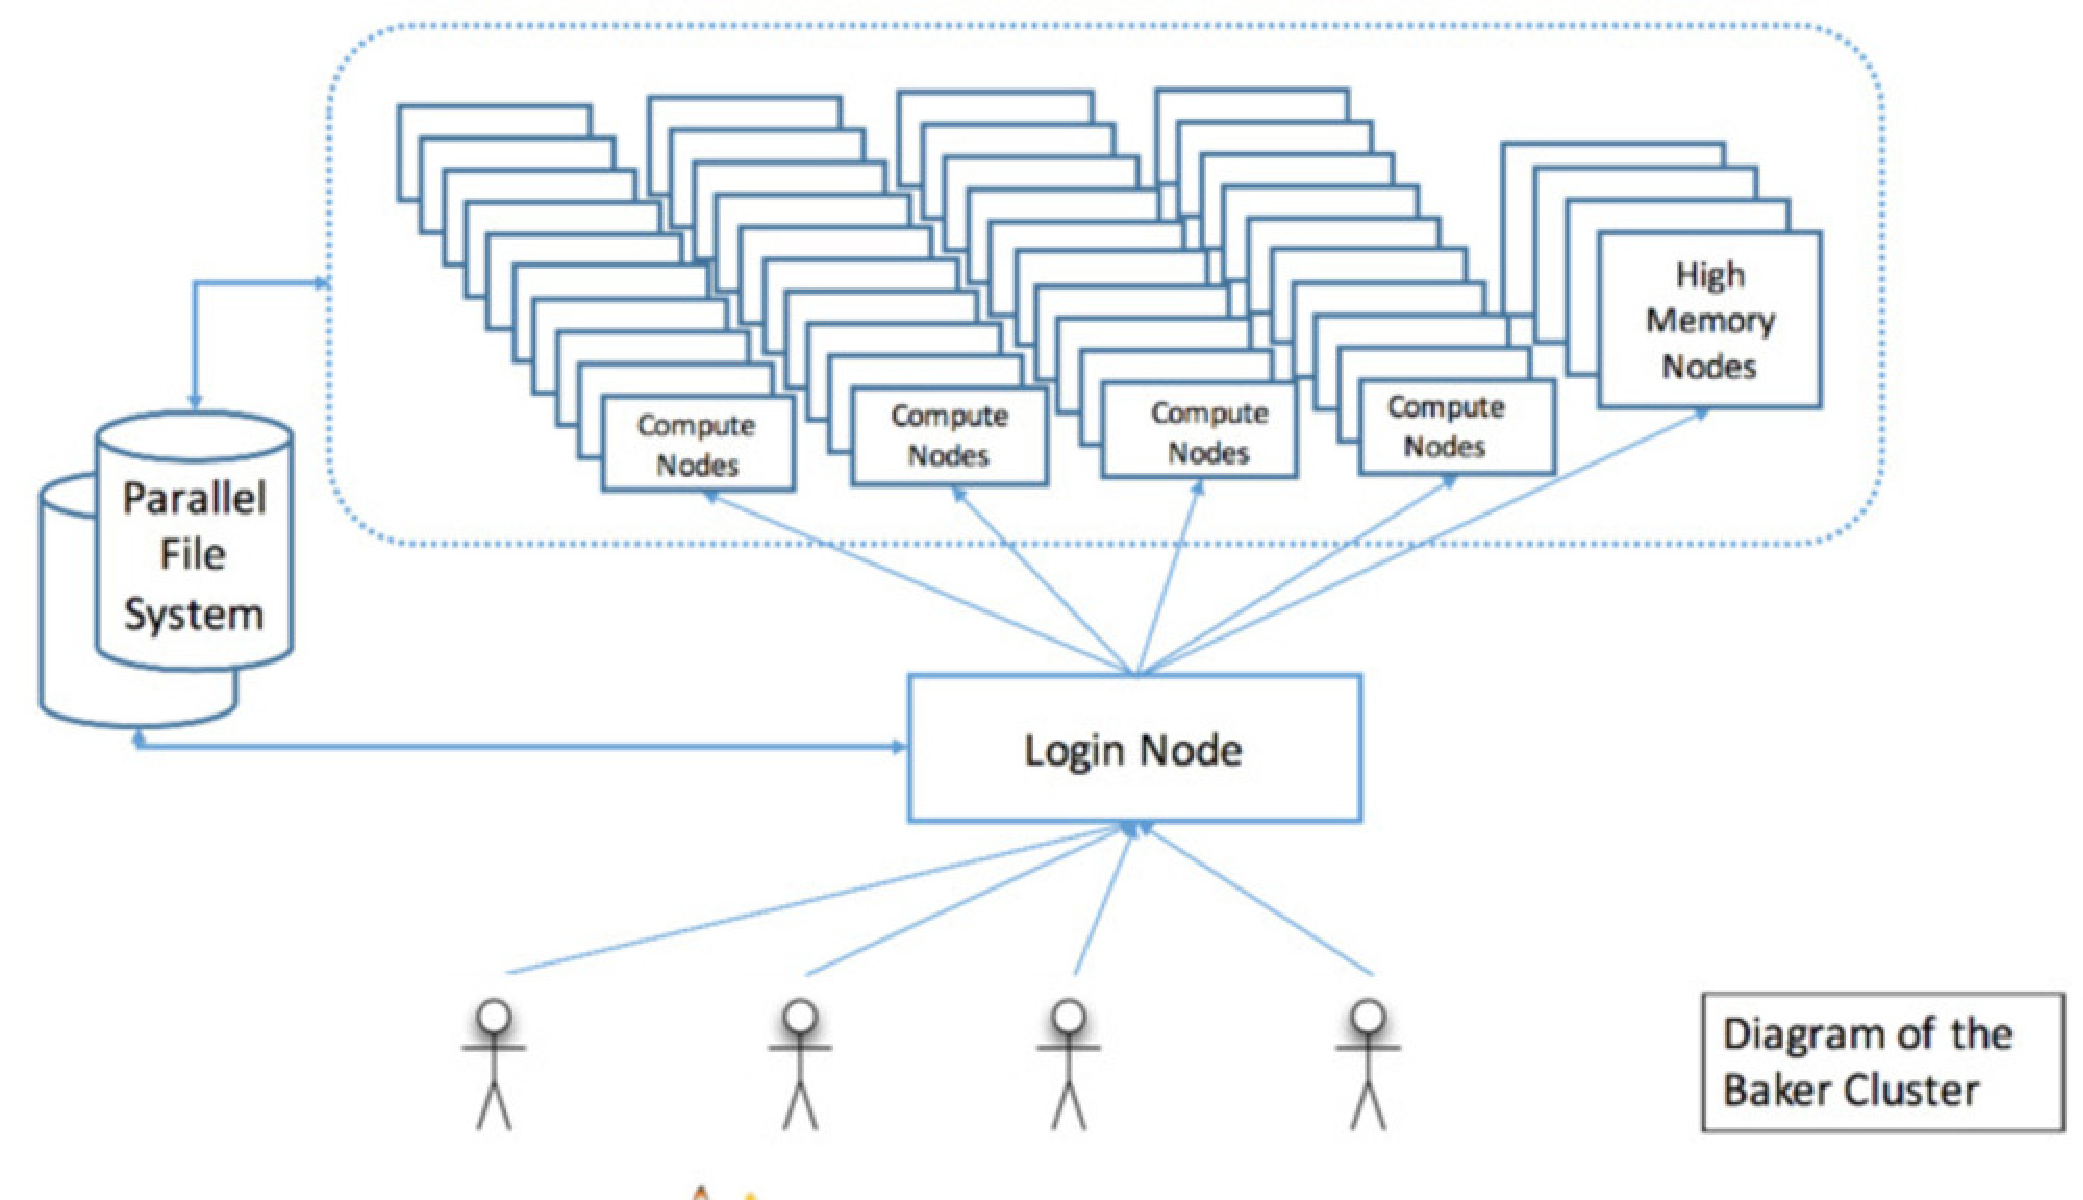
\includepdf{images/GPFS_File-eps-converted-to.pdf}
%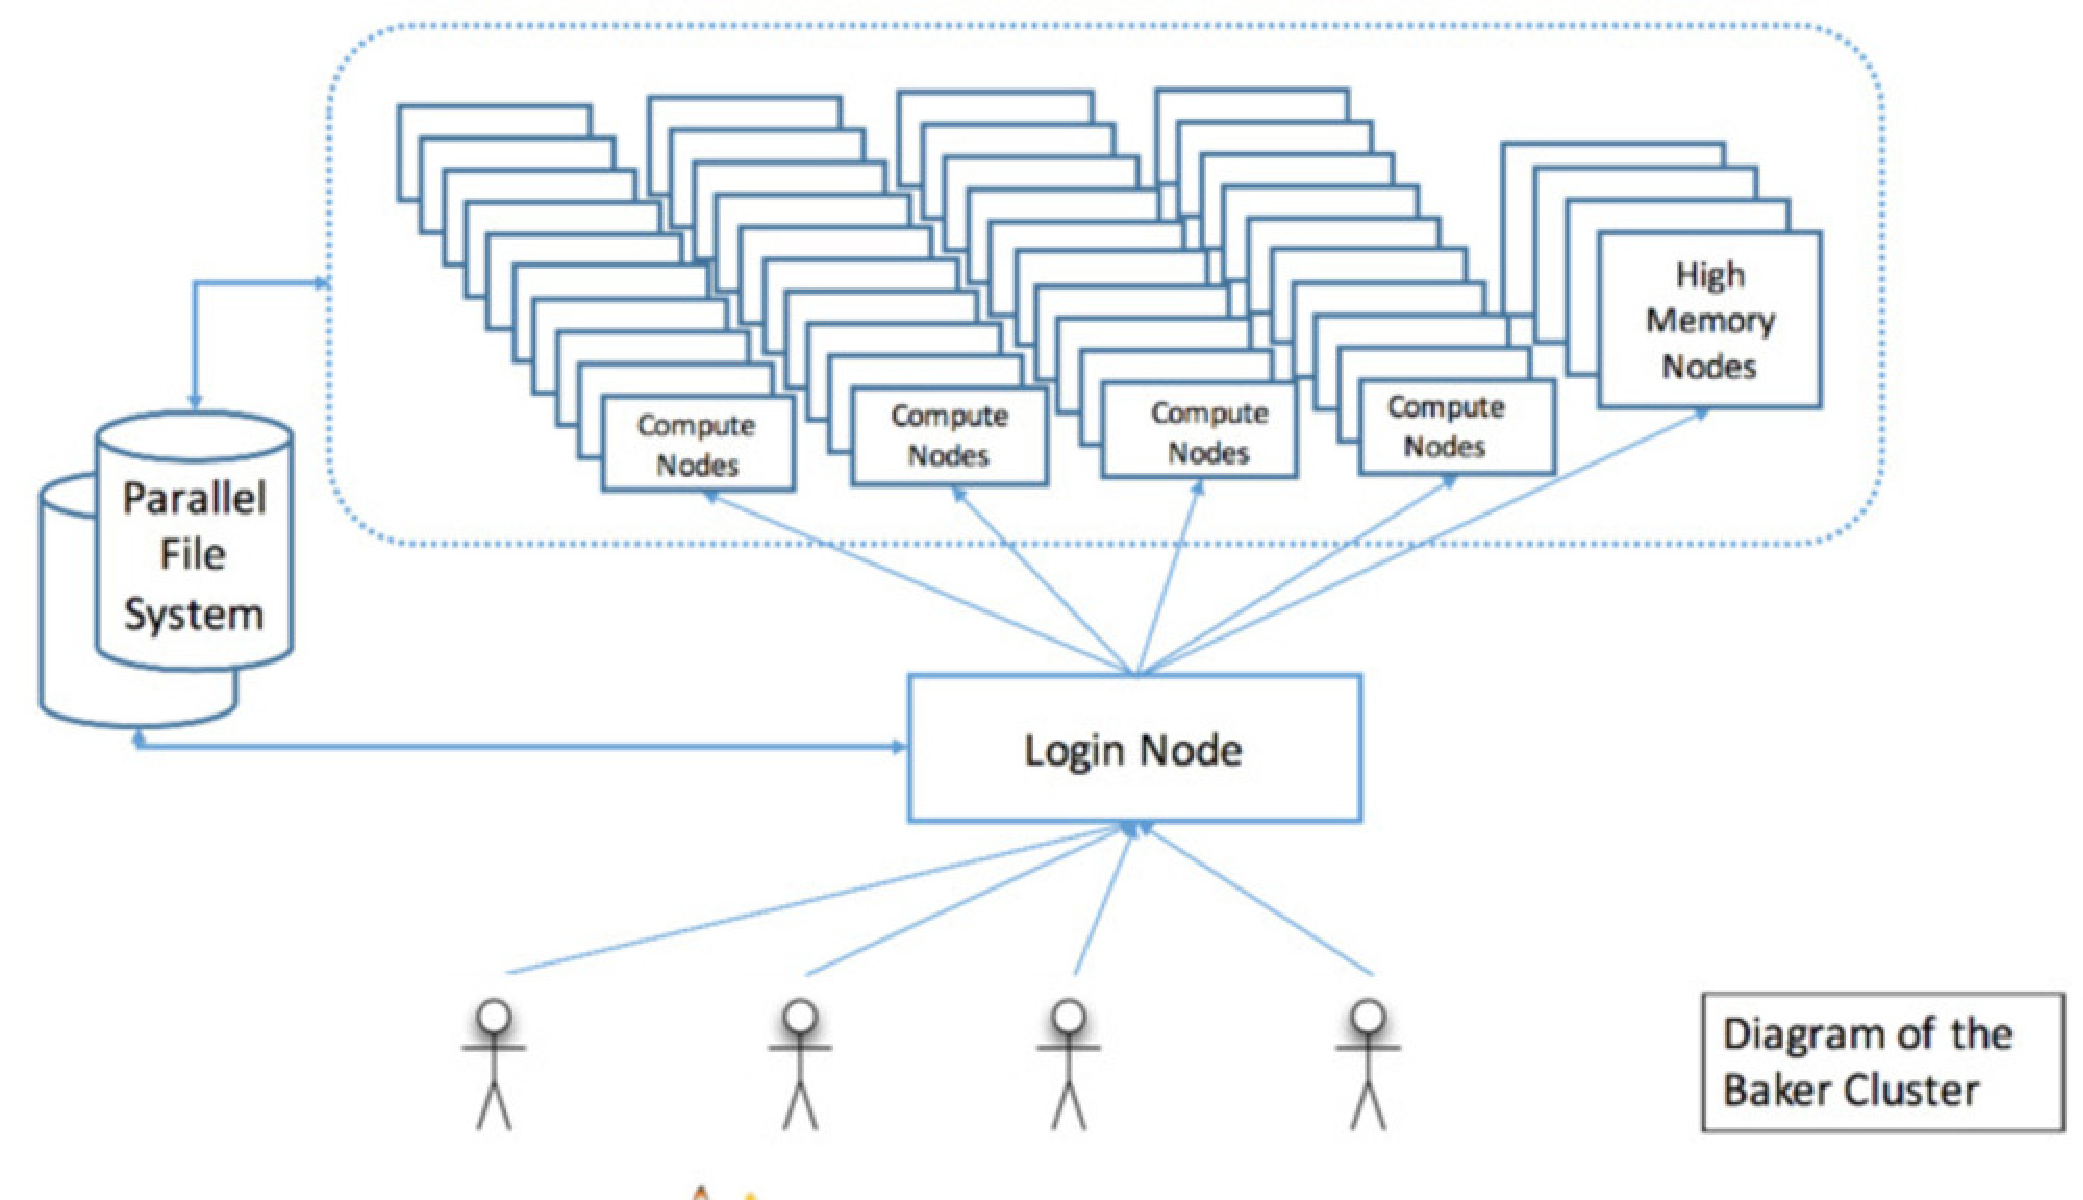
\includepdf{images/GPFS_File-eps-converted-to.pdf}

\put(0, 70){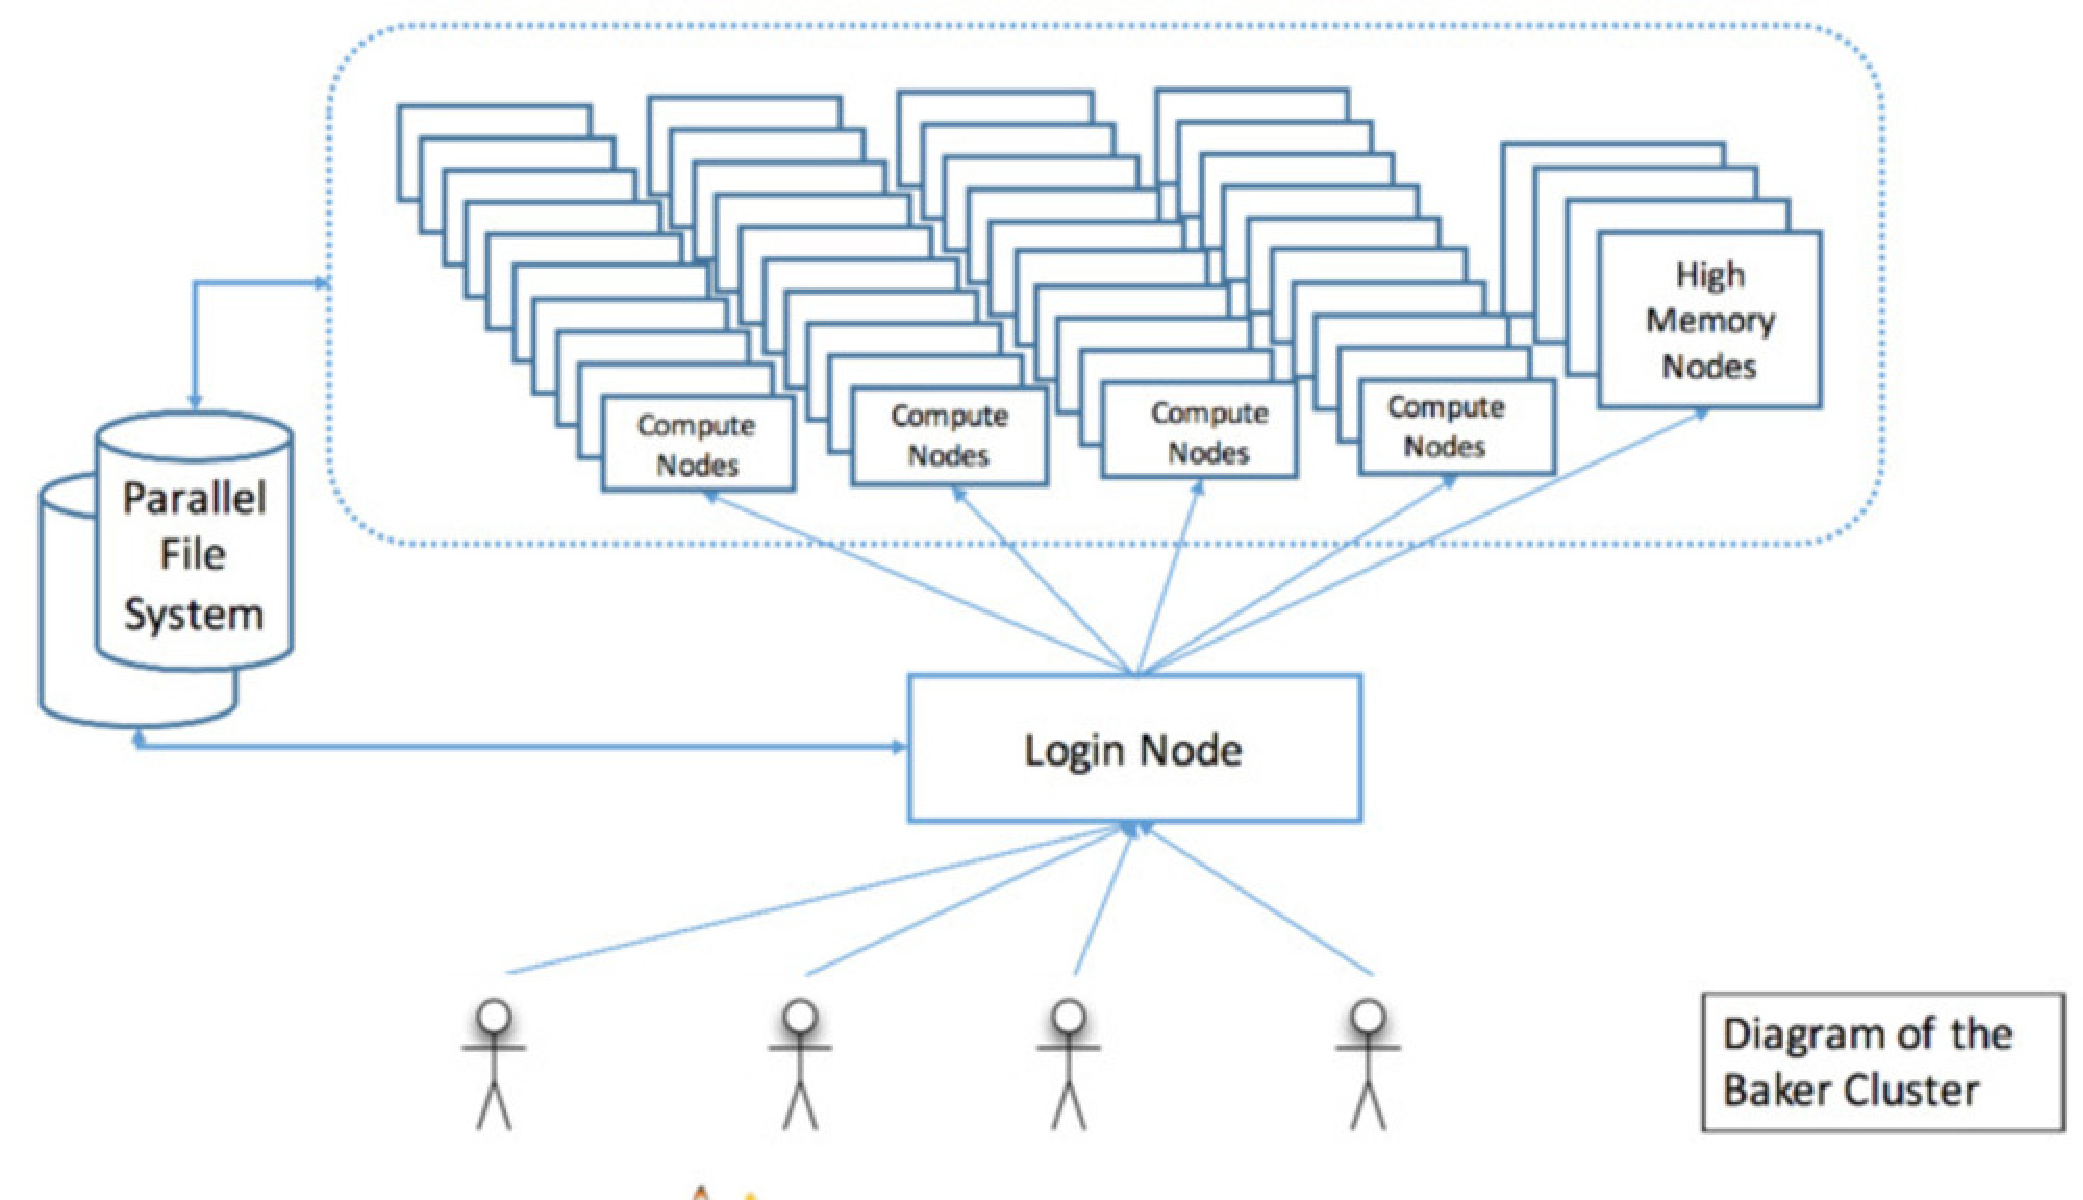
\includegraphics[height=2.5in]{images/GPFS_File-eps-converted-to.pdf}}
\end{picture}
\end{frame}


\begin{frame}
\frametitle{HPC Concepts}
Parallelization:
\begin{itemize}
    \item Shared memory
        \begin{enumerate}
            \item All memory used is within the same physical computer
            \pause
            \item Often used for 'embarrassingly parallizeable' problems
            \pause 
            \item Protocals 
                \begin{itemize}
                    \item C/Fortran : OpenMP
                    \item R : parapply package
                    \item Python : multiprocessing module
                \end{itemize}
        \end{enumerate}
    
    \pause
    \bigskip
    \item This is your interface with the computer cluster
\end{itemize}
\end{frame}
 



\begin{frame}
\frametitle{What is Slurm?}
A Workload Manager
\begin{itemize}
    \item Permits efficient (and fair) utilization of Cluster resources.
    \bigskip
    \item This is your interface with the computer cluster
\end{itemize}
\end{frame}
 

\begin{frame}
\frametitle{Slurm Concepts}
\begin{itemize}
    \item Job
    \pause 
    \begin{enumerate}
        \item Composed of one or more Steps
    \end{enumerate}
    \bigskip
    \pause
    \item Step
    \begin{enumerate}
        \item Composed of one or more Tasks
    \end{enumerate}
    \bigskip
    \pause
    \item Task
    \begin{enumerate}
        \item Composed of one or more CPUs
    \end{enumerate}
    \bigskip
\end{itemize}
\end{frame}


\begin{frame}
\frametitle{Baker}
A typical job on Baker : 
\begin{itemize}
    \item 1 Node 
    \pause 
    \bigskip
    \pause
    \item 1 Task
    \bigskip
    \pause
    \item Multiple CPUs
\end{itemize}
Complicated jobs may benefit from utilizing steps and tasks, most jobs will not.
\end{frame}


\begin{frame}
\frametitle{Baker}
Type of hardware available
\begin{itemize}
    \item High Memory (himem)
    \begin{enumerate}
        \item 1.5 TB RAM
        \item 48 cores 
        \item Ivy Bridge CPUs - slower memory access
    \end{enumerate}
    \pause 
    \bigskip
    \pause
    \item General Purpose (default)
    \begin{enumerate}
        \item 128 GB RAM
        \item 20 cores 
        \item Haswell - faster memory access
    \end{enumerate}
    \bigskip
    \pause
    \item GPU 
    \begin{enumerate}
        \item 128 GB and 192GB RAM 
        \item 20 cores 
        \item Haswell and ? CPUs
        \item NVidia K40, P100 and V100 available
    \end{enumerate}
\end{itemize}
\end{frame}



\begin{frame}
\frametitle{How to use Slurm?}
\begin{itemize}
    \item \code{sbatch} - Bash script
    \bigskip
    \pause
    \item \code{salloc} - Interactive sessions
    \bigskip
    \pause
    \item \code{srun-x11} - Interactive sessions - with x11 forwarding
    \bigskip
\end{itemize}
\end{frame}


\begin{frame}
\frametitle{\code{sbatch}}
Examples of Usage:
\begin{itemize}
    \item \code{sbatch myscript.sh}
    \bigskip
    \pause
    \item \code{sbatch --cpus-per-task=20 myscript.sh}
    \bigskip
    \pause
    \begin{enumerate}
        \item NOTE : specifying 20 cores, will not magically make your script use 20 cores.
                     You will need to specify that within your shell script \code{myscript.sh}
    \end{enumerate}
\end{itemize}


\end{frame}

\begin{frame}
\frametitle{\code{sbatch} - Bash script}
Two ways to pass arguments to sbatch
\begin{itemize}
    \item Command line
    \bigskip
    \pause
    \item 
    \bigskip
\end{itemize}
\end{frame}
% 
%
%\begin{frame}
%\frametitle{Types of Users}
%\begin{itemize}
%    \item Regular users (you)
%    \bigskip
%
%    \item Priveleged users (Yuan and myself)
%    \bigskip
%
%    \begin{itemize}
%        \item Can modify \code{/usr}, \code{/opt}, etc.
%        \bigskip
%
%        \item \code{sudo}
%    \end{itemize}
%\end{itemize}
%\end{frame}
%
%
%\begin{frame}
%\frametitle{The ``Shell"}
%%\begin{picture}(320,250)  %must be related to where it is centered
%%%\put(-30, 200){\includegraphics[height=0.8in]{images/Panoramic_Austin.jpg}}
%%\put(100, 100){\includegraphics[height=1.8in]{images/shell.eps}}
%%\end{picture}
%%\begin{tabular}{cl}  
%%  \begin{tabular}{c}
%%    \includegraphics[height=7cm, width=4.5cm]{images/shell.eps}
%%    \end{tabular}
%%    & \begin{tabular}{l}
%%      \parbox{0.5\linewidth}{%  change the parbox width as appropiate
%    \begin{itemize}
%        \item Used at the command line, i.e. the `terminal'
%        \bigskip
%        \item The user interface with the operating system
%        \bigskip
%        \item Bash is the default shell on Baker.
%    \end{itemize}
%%    }
%%    \end{tabular}  \\
%%\end{tabular}
%\end{frame}
%
%
%\begin{frame}
%\frametitle{Text Editors}
%\begin{itemize}
%    \item \code{vim}   : Command line based
%    \bigskip
%    \item \code{emacs} : Command line based
%    \bigskip
%    \item \code{gedit} : Graphical  based
%\end{itemize}
%\end{frame}
%
%%\begin{frame}
%%\begin{picture}(320,250)  %must be related to where it is centered
%%\put(20, 10){\includegraphics[height=3.5in, width=3.5in]{images/vim.eps}}
%%\end{picture}
%%\frametitle{Vim}
%%\end{frame}
%
%\begin{frame}
%\frametitle{Basic Commands}
%\code{vim} - text editor
%\bigskip
%\begin{itemize}
%    \item \code{vim $\sim$/Scatch/tmp.txt}
%    \bigskip
%    \item Command and Edit modes.
%    \bigskip
%    \item \code{esc} to enter command mode
%    \bigskip
%    \item \code{i} to enter edit mode
%    \bigskip
%    \item To save, in command mode : \code{esc} \code{:w}
%    \bigskip
%    \item To quit, in command mode : \code{esc} \code{:q}
%\end{itemize}
%\end{frame}
%
%\begin{frame}
%\frametitle{Basic Commands}
%\code{ls} - List directories and files. E.g.
%\bigskip
%\begin{itemize}
%    \item \code{ls /opt/python }
%    \bigskip
%
%    \item \code{ls -l /opt/python} 
%\end{itemize}
%\end{frame}
%
%
%
%\begin{frame}
%\frametitle{Basic Commands}
%\code{mkdir} - Make directories. E.g.
%\bigskip
%\begin{itemize}
%    \item \code{mkdir $\sim$/Scratch/newdir}
%\end{itemize}
%\end{frame}
%
%
%\begin{frame}
%\frametitle{Basic Commands}
%\code{man} - prints user manual for command. E.g.
%\bigskip
%\begin{itemize}
%    \item \code{man ls}
%    \bigskip
%    \item Use \code{d} and \code{b} to navigate forward and back.
%    \bigskip
%    \item Use \code{q} to quit
%    \bigskip
%    \item Use \code{/somestring} to search for \code{somestring} within the man page.
%\end{itemize}
%\end{frame}
%
%
%\begin{frame}
%\frametitle{Basic Commands}
%\code{cd}- Change directory. E.g.
%\bigskip
%\begin{itemize}
%    \item \code{cd $\sim$/Scratch}
%    \bigskip
%    \item \code{cd}
%    \bigskip
%    \item \code{cd ..}
%    \bigskip
%    \item \code{cd $\sim$} 
%\end{itemize}
%\end{frame}
%
%
%\begin{frame}
%\frametitle{Basic Commands}
%\code{pwd}- print working directory. E.g.
%\bigskip
%\begin{itemize}
%    \item \code{pwd}
%\end{itemize}
%\end{frame}
%
%
%\begin{frame}
%\frametitle{Basic Commands}
%\code{touch}- Create empty file. E.g.
%\bigskip
%\begin{itemize}
%    \item \code{touch $\sim$/Scratch/file.txt}
%\end{itemize}
%\end{frame}
%
%
%\begin{frame}
%\frametitle{Basic Commands}
%\code{mv}- move file or rename file. E.g.
%\bigskip
%\begin{itemize}
%    \item \code{mv $\sim$/Scratch/file.txt $\sim$/Scratch/file2.txt}
%\end{itemize}
%\end{frame}
%
%\begin{frame}
%\frametitle{Basic Commands}
%\code{cp}- copy files or directories
%\bigskip
%\begin{itemize}
%    \item \code{cp $\sim$/Scratch/file.txt $\sim$/Scratch/file2.txt}
%    \bigskip
%    \item \code{cp -r $\sim$/Scratch/newdir $\sim$/Scratch/newdir2}
%\end{itemize}
%\end{frame}
%
%
%\begin{frame}
%\frametitle{Basic Commands}
%\code{rm}- delete files or directories. Be Careful. E.g.
%\bigskip
%\begin{itemize}
%    \item \code{rm $\sim$/Scratch/file.txt}
%    \bigskip
%    \item \code{rm -r $\sim$/Scratch/newdir}
%\end{itemize}
%\end{frame}
%
%
%\begin{frame}
%\frametitle{Basic Commands}
%\code{cat}- concatenate files. E.g.
%\bigskip
%\begin{itemize}
%    \item \code{cat /opt/modulefiles/gcc-4.9.2}
%\end{itemize}
%\end{frame}
%
%
%\begin{frame}
%\frametitle{Basic Commands}
%\code{echo}- echo back string. E.g.
%\bigskip
%\begin{itemize}
%    \item \code{echo "Hello World"}
%\end{itemize}
%\end{frame}
%
%
%\begin{frame}
%\frametitle{Permissions}
%\code{chmod}- Change permissions.
%E.g.
%\begin{itemize}
%    \item \code{ls -l $\sim$/Scratch/file.txt}, yields : 
%    \hspace{5mm} \code{-rw-r--r--  1 user group 0 Apr  5 09:01 file.txt}
%    \smallskip
%    \item \code{chmod 755 somescript.sh}
%    \bigskip
%    \item \code{ls -l $\sim$/Scratch/file.txt}, yields : 
%    \hspace{5mm} \code{-rwxr-xr-x  1 user group 0 Apr  5 09:01 file.txt}
%\end{itemize}
%\bigskip
%
%Explanation:
%\begin{itemize}
%    \item First number is you.
%    \item Second number is for your group (i.e. lab).
%    \item Third number is for everyone else.
%    \item \code{r} = 4, \code{w} = 2, \code{x} = 1
%    \item \code{7} = \code{4} + \code{2} + \code{1} = read (\code{r}) + write (\code{w}) +  execute(\code{x})
%    \item \code{5} = \code{4} + \code{1} = read (\code{r}), execute(\code{x})
%\end{itemize}
%\end{frame}
%
%\begin{frame}
%\frametitle{Homework}
%Create a bash script that says ``Hello World". Make it executable. 
%
%\bigskip
%
%\emph{HINT}, you'll need to add $\code{\#^^21/bin/bash}$ at the top of your script
%\end{frame}

\end{document}





